\documentclass[nobib]{tufte-book}

\hypersetup{colorlinks}

\title{Introduction to Graph Theory: Exercises}
\author{Eric Bailey}
%% \publisher{Dover}

\usepackage{amssymb}

\usepackage{braket}

\usepackage{ebproof}

\usepackage{fancyvrb}
\fvset{fontsize=\normalsize}

%% \usepackage{makeidx}
%% \makeindex

\usepackage{mathtools}
\DeclarePairedDelimiter\abs{\lvert}{\rvert}

\usepackage{tikz}
\usepackage{tkz-berge}
%% \usepackage{tkz-graph}

\usepackage{todonotes}

%% \usepackage{xspace}

%% \newcommand{\blankpage}{\newpage\hbox{}\thispagestyle{empty}\newpage}

\newcommand{\powerset}[1]{\mathcal{P}\left(#1\right)}

\begin{document}

\frontmatter

%% \blankpage

\maketitle

\tableofcontents

%% \listoffigures

%% \listoftables

\mainmatter

\chapter{Graphs}
\label{ch:graphs}

\section{Exercises}

\begin{enumerate}
\item $\powerset{\Set{1,2,3}} \coloneqq \Set{
  \emptyset,
  \Set{1},    \Set{2},   \Set{3},
  \Set{1,2},  \Set{1,3}, \Set{2,3},
  \Set{1,2,3}
}$

\item
  \begin{prooftree*}
    \hypo{ \emptyset \nsubseteq A }
    \infer1{ \exists x \in \emptyset\ \colon x \not\in A }
    \infer0{ \neg \exists x \in \emptyset }
    \infer2{ \bot }
    \infer1{ \emptyset \subseteq A }
  \end{prooftree*}
  $\hfill\square$

\item
  \[
    \begin{prooftree}
      \infer0{ S(b) \coloneqq \Set{ m \in V \colon m \not\in S(m) } }
      \infer0{ b \in V }
      \infer2{ b \in S(b) \Leftarrow\!\Rightarrow b \not\in S(b) }
    \end{prooftree}
    \equiv
    \begin{prooftree}
      \infer0{ R = \Set{ x \not\in x } }
      \infer1{ R \in R \Leftarrow\!\Rightarrow R \not\in R }
    \end{prooftree}
  \]

\item Let $S$ be the collection of all sets that can be described in an English
  sentence of twenty-five words or less. $S$ is not a set, because $S$ can be
  described in fewer than twenty-five words, and if it were a set, then $S$
  would have to be a member of itself, which violates the axiomatic definition
  of a set.

\item
  \begin{figure*}
    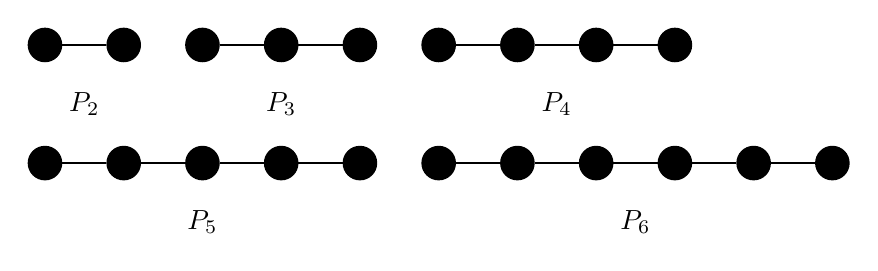
\begin{tikzpicture}[scale=.5]
      \GraphInit[vstyle=Simple]

      \begin{scope}
        \grPath[RA=2]{2}
        \draw (1,-1.5) node {$P_{2}$};
      \end{scope}

      \begin{scope}[xshift=4cm]
        \grPath[RA=2]{3}
        \draw (2,-1.5) node {$P_{3}$};
      \end{scope}

      \begin{scope}[xshift=10cm]
        \grPath[RA=2]{4}
        \draw (3,-1.5) node {$P_{4}$};
      \end{scope}

      \begin{scope}[yshift=-3cm]
        \grPath[RA=2]{5}
        \draw (4,-1.5) node {$P_{5}$};
      \end{scope}

      \begin{scope}[yshift=-3cm,xshift=10cm]
        \grPath[RA=2]{6}
        \draw (5,-1.5) node {$P_{6}$};
      \end{scope}
    \end{tikzpicture}
  \end{figure*}

  \begin{align*}
    V(P_{v})        &= \Set{ 1, 2, ..., v } \\
    E(P_{v})        &= \Set{ \Set{n-1,n} \colon n \in \Set{ 2, ..., v } } \\
    \abs*{E(P_{v})} &= v - 1 \\
    e               &= v - 1
  \end{align*}
  $\hfill\square$

  \marginnote[-6em]{%
    The number of edges in a {\em path graph} $P_{v}$, where $v \ge 2$, is
    given by the formula $e = v - 1$.%
  }
  \newpage

\item
  \begin{figure*}
    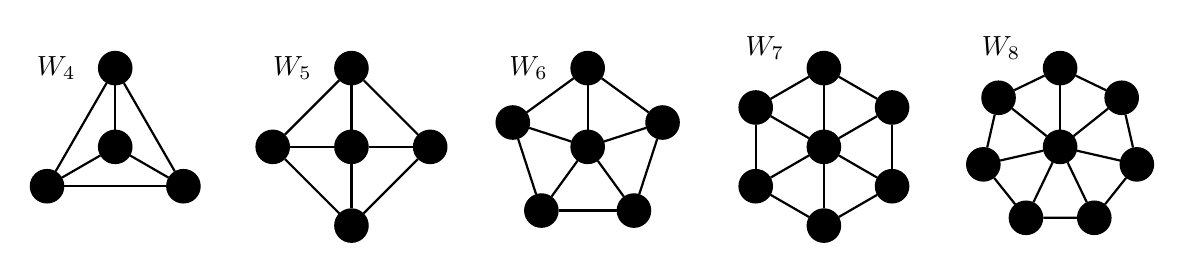
\begin{tikzpicture}[scale=.5]
      \GraphInit[vstyle=Simple]

      \begin{scope}[rotate=90]
        \grWheel[RA=2]{4}
        \draw (2,1.5) node {$W_{4}$};
      \end{scope}

      \begin{scope}[xshift=6cm]
        \grWheel[RA=2]{5}
        \draw (-1.5,2) node {$W_{5}$};
      \end{scope}

      \begin{scope}[xshift=12cm,rotate=90]
        \grWheel[RA=2]{6}
        \draw (2,1.5) node {$W_{6}$};
      \end{scope}

      %% \begin{scope}[xshift=3cm,yshift=-6cm,rotate=90]
      \begin{scope}[xshift=18cm,rotate=90]
        \grWheel[RA=2]{7}
        \draw (2.5,1.5) node {$W_{7}$};
      \end{scope}

      %% \begin{scope}[xshift=9cm,yshift=-6cm,rotate=90]
      \begin{scope}[xshift=24cm,rotate=90]
        \grWheel[RA=2]{8}
        \draw (2.5,1.5) node {$W_{8}$};
      \end{scope}
    \end{tikzpicture}
  \end{figure*}

  \begin{equation*}
    \begin{split}
      V(W_{v})        &= \Set{ 1, 2, 3, ..., v } \\
      E(W_{v})        &= \{\ \Set{1,2}, \Set{1,3}, ..., \Set{1,v}, \\
                      & \qquad \Set{2,3}, \Set{3,4}, ..., \Set{v-1,v}, \\
                      & \qquad \Set{v,2}\ \} \\
                      &= \{\ \Set{ \Set{1,n} \colon n \in \Set{2,...,v} }, \\
                      & \qquad \Set{ \Set{n-1,n} \colon n \in \Set{3,...,v} }, \\
                      & \qquad \Set{v,2}\ \} \\
      \abs*{E(W_{v})} &= (v-1) + (v-2) + 1 \\
                      & = (v-1) + (v-1) \\
      e               & = 2(v-1)
    \end{split}
  \end{equation*}
  $\hfill\square$

  \marginnote[-11em]{%
    The number of edges in {\em the wheel graph on $v$ vertices} $W_{v}$, where
    $v \ge 4$, is given by the formula $e = 2(v - 1)$.%
  }
  \newpage

\item
  \begin{align*}
    1 + 2 + ... + (v-1) &= (1/2)v(v-1) \\
    &= E(K_{v}) & \text{(T2)} \\
    &= (v-1) + (v-2) + ... + (v - (v-1)) \\
    &= 1 + 2 + ... (v-1)
  \end{align*}

  Imagine drawing $K_{v}$ by joining vertex $1$ to vertices $2$ through $v$,
  creating $v-1$ edges; then joining vertex $2$ to vertices $3$ through $v$,
  creating $v-2$ edges; and so on, i.e.
  $(v - 1) + (v - 2) + ... + (v - (v - 1))$, or equivalently,
  $1 + 2 + ... + (v - 1)$.
  $\hfill\square$

  \item \todo{p57}
\end{enumerate}

%% \backmatter

%% \printindex

\end{document}
